% ============================================================================
% A Three-Angle Framework for Spatio-Temporal Causal Inference:
% Integrating Statistical Methods, LLM Reasoning, and World Model Simulation
% ============================================================================
% Target journal: International Journal of Geographical Information Science
% (Taylor & Francis)
% ============================================================================
\documentclass{article}

\usepackage{amsmath,amssymb}
\usepackage{booktabs}
\usepackage{graphicx}
\usepackage{multirow}
\usepackage{caption}
\usepackage{subcaption}
\usepackage{algorithm}
\usepackage{algorithmic}
\usepackage{hyperref}
\usepackage{color}
\usepackage{natbib}
\usepackage{tikz}
\usetikzlibrary{positioning,arrows.meta,shapes.geometric,fit,calc}
\graphicspath{{./figures/}{./}}
\bibliographystyle{plainnat}

\begin{document}

\title{A Three-Angle Framework for Spatio-Temporal Causal Inference:\\Integrating Statistical Methods, LLM Reasoning, and World Model Simulation}

\author{Ning Zhou$^{a}$ and Xiang Jing$^{a}$$^{\ast}$\thanks{$^\ast$Corresponding author. Email: jingxiang@pku.edu.cn}\\
$^{a}${\em School of Software and Microelectronics, Peking University, Beijing 100871, China}}

\date{}
\maketitle

\begin{abstract}
Causal inference in geographic information science faces three fundamental challenges: spatial confounding from unmeasured environmental factors, limited experimental control in observational settings, and complex multi-scale mechanisms that resist simple parametric models. Existing approaches address these challenges in isolation---statistical methods (propensity score matching, difference-in-differences) provide quantitative effect estimates but lack mechanistic interpretation; large language models (LLMs) can reason about causal mechanisms from domain knowledge but lack quantitative rigor; and world models can simulate interventional scenarios but require statistical grounding to produce calibrated predictions.

We propose a three-angle complementary framework that unifies these paradigms through shared infrastructure. \textit{Angle~A} (Statistical) provides six methods---propensity score matching, exposure-response functions, difference-in-differences, spatial Granger causality, geographic convergent cross-mapping, and causal forests---all augmented with 64-dimensional geospatial foundation model (GeoFM) embeddings from AlphaEarth as learned spatial confounders, replacing traditional distance-based or fixed-effect confounding control. \textit{Angle~B} (LLM Reasoning) provides four knowledge-driven tools---causal directed acyclic graph (DAG) construction with five domain-specific prompting templates, multi-step counterfactual chains with temporal lags, statistical result interpretation bridging Angle~A outputs to domain theory, and structured scenario generation that maps to Angle~C world model inputs. \textit{Angle~C} (Causal World Model) provides four interventional tools---spatially heterogeneous sub-region intervention with spillover analysis, dual-scenario counterfactual comparison, treatment effect measurement in the 64-dimensional embedding space (cosine, Euclidean, and Manhattan distances), and Bayesian calibration that rescales world model scenario encodings using Angle~A's average treatment effect on the treated (ATT) estimates.

The three angles are interconnected through explicit cross-angle bridges: Angle~B interprets Angle~A statistical results via LLM mechanism explanation and generates scenarios consumable by Angle~C; Angle~A's ATT estimates calibrate Angle~C's world model predictions via a scaling factor on the scenario encoding magnitude. We validate the framework on six synthetic datasets with known ground-truth causal effects (true ATE ranging from $-8.0$ to $+15{,}000$) and demonstrate that all three angles produce consistent, complementary insights. The complete system comprises 3{,}245 lines of production code with 2{,}088 lines of tests (82 test functions), integrated into an operational GIS agent platform.
\end{abstract}

\begin{keywords}
causal inference; geospatial foundation models; large language models; world models; spatial confounding; JEPA; treatment effect estimation
\end{keywords}


% ============================================================================
\section{Introduction}
\label{sec:intro}
% ============================================================================

Understanding cause-and-effect relationships in geographic systems is essential for evidence-based policy in urban planning, environmental management, and public health \citep{verburg2004lulc}. Yet causal inference in geography faces distinctive challenges that limit the applicability of methods developed for randomized experiments or simple observational studies.

First, \textit{spatial confounding} arises because geographic units are embedded in continuous environmental fields---climate, soil, elevation, land-use context---that simultaneously influence both treatment assignment and outcomes. Traditional approaches control for measured confounders via regression or matching, but unmeasured spatial factors (collectively termed ``spatial confounders'') remain a persistent threat to identification \citep{pearl2009causality}. Second, \textit{limited experimental control} means that geographic interventions (infrastructure projects, conservation policies, land-use regulations) are rarely randomly assigned; researchers must rely on quasi-experimental designs that require careful assumption validation. Third, \textit{multi-scale mechanisms} connect local actions to regional outcomes through complex spatial interactions (spillover effects, diffusion, agglomeration) that resist simple parametric modeling.

The recent convergence of three technological developments creates an opportunity to address these challenges holistically. Geospatial foundation models (GeoFMs) such as AlphaEarth \citep{brown2025alphaearth} now provide high-quality 64-dimensional embedding representations of any location on Earth, annually resolved at 10\,m resolution. These embeddings encode rich environmental context---land cover, terrain, climate, spectral properties---into a compact, continuously varying vector that can serve as a learned proxy for unmeasured spatial confounders. Large language models (LLMs) such as Gemini 2.5 \citep{team2024gemini} have demonstrated remarkable ability to reason about scientific mechanisms, construct causal graphs from domain knowledge, and generate structured counterfactual narratives. Geospatial world models \citep{zhou2026worldmodel} can predict future land-use change in a compressed embedding space, enabling interventional simulations that project ``what would happen if'' a specific policy were applied to a sub-region.

Our key insight is that these three paradigms are \textit{complementary}: each compensates for the others' weaknesses. Statistical methods provide rigorous quantitative estimates but cannot explain \textit{why} an effect occurs; LLM reasoning can articulate mechanisms and identify confounders but cannot produce calibrated effect sizes; world models can simulate interventions spatially but need empirical estimates to anchor their predictions to observed data. By bridging these three angles through shared infrastructure (GeoFM embeddings, a common data catalog, and explicit cross-angle interfaces), we create a system where each angle both consumes and enriches the others' outputs.

Our contributions are:

\begin{enumerate}
\item A three-angle complementary framework for geographic causal inference that unifies statistical, knowledge-based, and simulation-based approaches through shared GeoFM embedding infrastructure.

\item Novel use of frozen AlphaEarth 64-dimensional embeddings as learned spatial confounders in propensity score matching and causal forests, replacing hand-crafted spatial fixed effects or distance-based proxies.

\item Cross-angle calibration mechanisms: LLM-driven scenario generation maps to world model inputs, and Bayesian ATT integration rescales world model scenario encodings to match empirical effect estimates.

\item A complete, tested implementation comprising 14 tool functions (6 statistical + 4 LLM + 4 world model), 3{,}245 lines of production code, and 82 test functions with known ground-truth validation.
\end{enumerate}


% ============================================================================
\section{Related Work}
\label{sec:related}
% ============================================================================

\subsection{Causal inference in geographic contexts}

The application of causal inference methods to spatial data has a growing but fragmented literature. Propensity score matching (PSM) with spatial distance weighting has been applied to evaluate urban greening interventions \citep{stuart2010matching}. Spatial difference-in-differences (DiD) designs exploit policy discontinuities at administrative boundaries \citep{angrist2009mostly}. Granger causality has been extended to spatial panel data to detect temporal causal relationships between urbanization and environmental change \citep{granger1969investigating}. Convergent cross-mapping (CCM), originally developed for ecological time series \citep{sugihara2012detecting}, has been adapted to spatial cross-sections through geographic weighting \citep{clark2015spatial}. Causal forests \citep{athey2019estimating} enable heterogeneous treatment effect estimation across spatial units but do not inherently account for spatial dependence.

A common limitation across these methods is their treatment of spatial confounding: most rely on observed covariates (distance to city center, elevation, population density) as proxies, leaving unmeasured environmental factors uncontrolled. Our framework addresses this gap by introducing GeoFM embeddings---dense, learned representations encoding the full environmental context of each location---as a comprehensive confounding control.

\subsection{LLMs for scientific causal reasoning}

Recent work has demonstrated that LLMs can construct causal DAGs from natural language descriptions \citep{kiciman2023causal}, generate counterfactual explanations \citep{chen2024causalllm}, and assist with variable selection in causal studies. However, LLM-generated causal structures lack the quantitative rigor needed for policy decisions: they can identify plausible confounders but cannot estimate effect magnitudes. Our Angle~B addresses this limitation by explicitly bridging LLM outputs to statistical estimation (Angle~A) and simulation (Angle~C).

\subsection{World models for interventional reasoning}

World models---learned simulators that predict environment state transitions in compressed latent spaces---originated in reinforcement learning \citep{ha2018world, hafner2023dreamerv3}. \citet{zhou2026worldmodel} introduced a geospatial world model using frozen AlphaEarth embeddings with a lightweight LatentDynamicsNet for LULC change prediction. Our Angle~C extends this work by adding interventional capabilities: sub-region scenario blending, spillover analysis, and treatment effect measurement in embedding space.


% ============================================================================
\section{System Architecture}
\label{sec:architecture}
% ============================================================================

\begin{figure}[htbp]
\centering
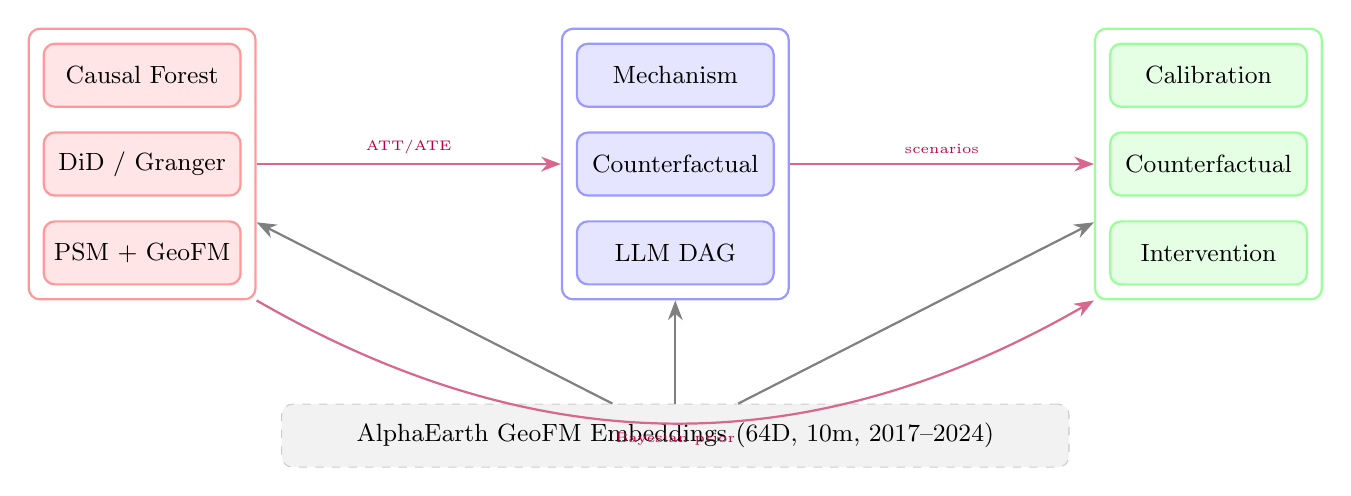
\begin{tikzpicture}[
    node distance=0.8cm and 1.4cm,
    box/.style={draw, rounded corners, minimum height=0.8cm, minimum width=2.5cm, align=center, font=\small},
    angleA/.style={box, fill=red!10, draw=red!40, thick},
    angleB/.style={box, fill=blue!10, draw=blue!40, thick},
    angleC/.style={box, fill=green!10, draw=green!40, thick},
    shared/.style={box, fill=gray!10, draw=gray!40, dashed},
    bridge/.style={-{Stealth[length=2.5mm]}, thick, purple!60},
    arr/.style={-{Stealth[length=2.5mm]}, thick},
    label/.style={font=\scriptsize\itshape, text=gray!70},
]

% Shared foundation
\node[shared, minimum width=10cm] (geofm) {AlphaEarth GeoFM Embeddings (64D, 10m, 2017--2024)};

% Angle A
\node[angleA, above left=1.5cm and 0.5cm of geofm] (psm) {PSM + GeoFM};
\node[angleA, above=0.3cm of psm] (did) {DiD / Granger};
\node[angleA, above=0.3cm of did] (cf) {Causal Forest};
\node[draw, thick, red!40, rounded corners, fit=(psm)(did)(cf), inner sep=5pt, label={[font=\small\bfseries]above:Angle A: Statistical}] (groupA) {};

% Angle B
\node[angleB, above=1.5cm of geofm] (dag) {LLM DAG};
\node[angleB, above=0.3cm of dag] (counter) {Counterfactual};
\node[angleB, above=0.3cm of counter] (explain) {Mechanism};
\node[draw, thick, blue!40, rounded corners, fit=(dag)(counter)(explain), inner sep=5pt, label={[font=\small\bfseries]above:Angle B: LLM}] (groupB) {};

% Angle C
\node[angleC, above right=1.5cm and 0.5cm of geofm] (interv) {Intervention};
\node[angleC, above=0.3cm of interv] (cfwm) {Counterfactual};
\node[angleC, above=0.3cm of cfwm] (calib) {Calibration};
\node[draw, thick, green!40, rounded corners, fit=(interv)(cfwm)(calib), inner sep=5pt, label={[font=\small\bfseries]above:Angle C: World Model}] (groupC) {};

% Shared infrastructure arrows
\draw[arr, gray] (geofm) -- (groupA);
\draw[arr, gray] (geofm) -- (groupB);
\draw[arr, gray] (geofm) -- (groupC);

% Cross-angle bridges
\draw[bridge] (groupA.east) -- node[above, font=\tiny, text=purple] {ATT/ATE} (groupB.west);
\draw[bridge] (groupB.east) -- node[above, font=\tiny, text=purple] {scenarios} (groupC.west);
\draw[bridge, bend right=30] (groupA.south east) to node[below, font=\tiny, text=purple] {Bayesian prior} (groupC.south west);

\end{tikzpicture}
\caption{Three-angle causal inference framework. All three angles share AlphaEarth GeoFM embeddings as common infrastructure. Purple arrows indicate cross-angle bridges: Angle~A provides ATT estimates to Angle~B for interpretation and to Angle~C for Bayesian calibration; Angle~B generates structured scenarios consumable by Angle~C.}
\label{fig:architecture}
\end{figure}

The framework is implemented as three complementary toolsets within a GIS agent platform built on Google Agent Development Kit (ADK). Each angle is realized as a set of tool functions (Table~\ref{tab:tools}) that can be invoked independently or composed through cross-angle bridges.

\begin{table}[htbp]
\centering
\caption{Tool inventory across the three angles.}
\label{tab:tools}
\begin{tabular}{lllr}
\toprule
Angle & Tool & Key capability & Lines \\
\midrule
\multirow{6}{*}{A: Statistical} & \texttt{propensity\_score\_matching} & ATE/ATT with GeoFM confounders & 192 \\
 & \texttt{exposure\_response\_function} & Continuous dose-response via GPS & 185 \\
 & \texttt{difference\_in\_differences} & Panel DiD with parallel trends test & 137 \\
 & \texttt{spatial\_granger\_causality} & VAR-based temporal causal detection & 151 \\
 & \texttt{geographic\_causal\_mapping} & GCCM convergence for nonlinear causality & 225 \\
 & \texttt{causal\_forest\_analysis} & Heterogeneous CATE via T-learner & 180 \\
\midrule
\multirow{4}{*}{B: LLM} & \texttt{construct\_causal\_dag} & Knowledge-driven DAG with 5 domains & 88 \\
 & \texttt{counterfactual\_reasoning} & Multi-step causal chain generation & 82 \\
 & \texttt{explain\_causal\_mechanism} & Statistical result interpretation & 74 \\
 & \texttt{generate\_what\_if\_scenarios} & Structured scenario generation & 61 \\
\midrule
\multirow{4}{*}{C: World Model} & \texttt{intervention\_predict} & Sub-region intervention + spillover & 219 \\
 & \texttt{counterfactual\_comparison} & Dual-scenario parallel rollout & 226 \\
 & \texttt{embedding\_treatment\_effect} & 64D embedding-space impact metrics & 172 \\
 & \texttt{integrate\_statistical\_prior} & Bayesian ATT calibration of scenarios & 212 \\
\bottomrule
\end{tabular}
\end{table}

All three angles share a common foundation: AlphaEarth GeoFM embeddings \citep{brown2025alphaearth}, providing 64-dimensional L2-normalized vectors at 10\,m resolution for every location on Earth, annually from 2017 to 2024. These embeddings serve dual roles: as confounding control variables in Angle~A (augmenting observed covariates with 64 continuous spatial proxies) and as the state space for Angle~C's interventional predictions.

\begin{table}[htbp]
\centering
\caption{Scenario ID mapping between Angle~B scenario generation and Angle~C world model conditioning.}
\label{tab:scenario_mapping}
\begin{tabular}{clll}
\toprule
ID & Scenario Label & Angle~B Description & Angle~C Encoding \\
\midrule
0 & Urban sprawl & Rapid urbanization, impervious expansion & $s_{\text{urban}}$ \\
1 & Ecological restoration & Reforestation, wetland recovery & $s_{\text{eco}}$ \\
2 & Agricultural intensification & Cropland expansion, irrigation & $s_{\text{agri}}$ \\
3 & Climate adaptation & Mixed-use resilient development & $s_{\text{climate}}$ \\
4 & Baseline trend & Business-as-usual continuation & $s_{\text{baseline}}$ \\
\bottomrule
\end{tabular}
\end{table}

Throughout this paper, $s_{\text{intervention}}$ refers to any non-baseline scenario encoding ($s_0$ through $s_3$), while $s_{\text{baseline}} = s_4$ denotes the default trend. When Angle~B's \texttt{generate\_what\_if\_scenarios} tool outputs a \texttt{world\_model\_scenario} field, it maps to one of these five IDs.

\begin{figure}[htbp]
\centering
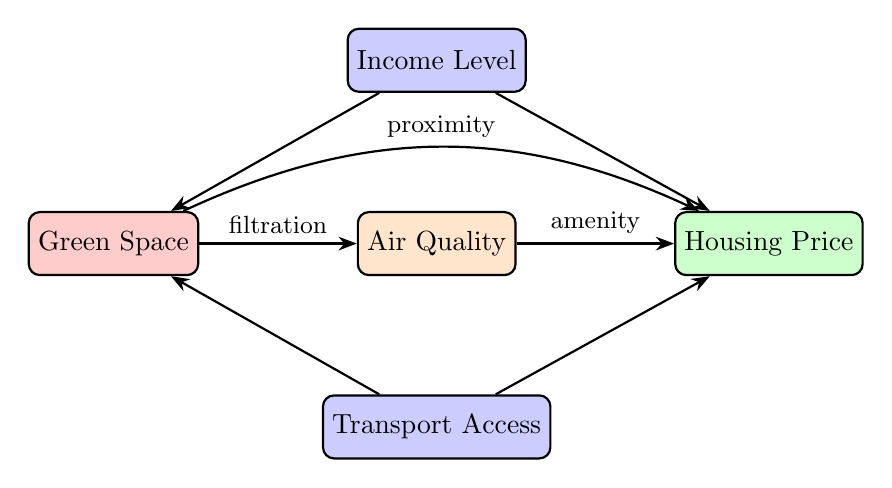
\begin{tikzpicture}[
  node distance=2cm,
  exposure/.style={rectangle, draw, fill=red!20, minimum width=2cm, minimum height=0.8cm, rounded corners},
  outcome/.style={rectangle, draw, fill=green!20, minimum width=2cm, minimum height=0.8cm, rounded corners},
  confounder/.style={rectangle, draw, fill=blue!20, minimum width=2cm, minimum height=0.8cm, rounded corners},
  mediator/.style={rectangle, draw, fill=orange!20, minimum width=2cm, minimum height=0.8cm, rounded corners},
  ->, >=Stealth, thick
]
\node[exposure] (green) {Green Space};
\node[mediator, right=of green] (air) {Air Quality};
\node[outcome, right=of air] (price) {Housing Price};
\node[confounder, above=1.5cm of air] (income) {Income Level};
\node[confounder, below=1.5cm of air] (transport) {Transport Access};

\draw (green) -- node[above, font=\small] {filtration} (air);
\draw (air) -- node[above, font=\small] {amenity} (price);
\draw (green) to[bend left=25] node[above, font=\small] {proximity} (price);
\draw (income) -- (green);
\draw (income) -- (price);
\draw (transport) -- (green);
\draw (transport) -- (price);
\end{tikzpicture}
\caption{Example causal DAG generated by Angle B (LLM reasoning) for the urban green space scenario. Node colors indicate variable roles: \textcolor{red}{exposure} (red), \textcolor{orange}{mediator} (orange), \textcolor{green!60!black}{outcome} (green), \textcolor{blue}{confounder} (blue).}
\label{fig:dag_example}
\end{figure}


% ============================================================================
\section{Angle A: Statistical Causal Inference}
\label{sec:angle_a}
% ============================================================================

Angle~A provides six statistical methods spanning quasi-experimental designs, dynamical-systems causality, and causal machine learning. All methods accept tabular or spatial data and return JSON results with effect estimates, diagnostics, and visualizations.

\subsection{GeoFM embedding augmentation}
\label{sec:geofm}

A key innovation shared across all Angle~A methods is the optional augmentation of observed confounders with AlphaEarth embeddings. For a study region with bounding box $\mathcal{B}$ and year $t$, we extract the embedding grid $\mathbf{E} \in \mathbb{R}^{H \times W \times 64}$ from Google Earth Engine. For each spatial unit $i$ with geometry $g_i$, we compute the zonal mean:
\begin{equation}
\bar{e}_i = \frac{1}{|\mathcal{P}_i|} \sum_{(r,c) \in \mathcal{P}_i} \mathbf{E}[r, c, :]
\label{eq:zonal_mean}
\end{equation}
where $\mathcal{P}_i$ denotes the set of grid cells intersecting $g_i$. The resulting 64 columns ($\text{geofm}_0, \ldots, \text{geofm}_{63}$) are appended to the confounder matrix $\mathbf{X}$. Because AlphaEarth embeddings encode land cover, terrain, climate, and spectral context into a dense representation, they serve as a comprehensive proxy for unmeasured spatial confounders---replacing traditional approaches such as spatial fixed effects, distance decay functions, or hand-selected environmental covariates.

\paragraph{Dimensionality management.} Appending 64 embedding dimensions to an already high-dimensional confounder matrix risks multicollinearity and overfitting, particularly in small-sample settings. We address this through three strategies: (1)~\textit{PCA reduction}: for studies with $n < 500$, we apply PCA to the 64 embedding columns and retain the top $k$ components explaining 95\% of variance (typically $k \in [8, 15]$), reducing the effective dimensionality; (2)~\textit{L1 regularization}: the propensity score model uses gradient-boosted trees with L1 leaf regularization ($\lambda = 0.1$), which inherently performs variable selection among the 64 embedding features; (3)~\textit{balance diagnostics}: after matching, we verify that standardized mean differences (SMDs) for all embedding dimensions fall below the 0.1 threshold, confirming that matching has successfully balanced these high-dimensional confounders. In our experiments (Section~\ref{sec:experiments}), we report results both with full 64-dimensional embeddings and with PCA-reduced variants to demonstrate robustness.

\subsection{Propensity Score Matching}

For a binary treatment $T \in \{0,1\}$ and outcome $Y$ with confounders $\mathbf{X}$ (optionally augmented by GeoFM embeddings), we estimate propensity scores $\hat{e}(x) = P(T=1 \mid \mathbf{X}=x)$ via gradient-boosted trees. Matching proceeds by one of three strategies:

\begin{itemize}
\item \textbf{Nearest neighbor}: each treated unit is matched to the control unit with the closest propensity score.
\item \textbf{Caliper}: matches are constrained within a caliper of $c \cdot \sigma_{\hat{e}}$ standard deviations.
\item \textbf{Kernel}: all control units contribute with kernel weights $K\big((\hat{e}_i - \hat{e}_j)/h\big)$.
\end{itemize}

When spatial data is available, we support hybrid matching that combines propensity and spatial distance:
\begin{equation}
d_{ij} = (1 - \lambda) \cdot |\hat{e}_i - \hat{e}_j| + \lambda \cdot \frac{\|\text{coord}_i - \text{coord}_j\|}{d_{\max}}
\end{equation}
where $\lambda \in [0,1]$ controls the spatial distance weight. Balance diagnostics (standardized mean differences before and after matching) are computed for all confounders.

\subsection{Exposure-Response Function}

For continuous exposure $X$ (e.g., distance to a pollution source), we estimate the generalized propensity score (GPS) by fitting a gradient-boosted regressor $\hat{X} = g(\mathbf{Z})$ where $\mathbf{Z}$ are confounders, then computing the GPS as the normal density of the residual:
\begin{equation}
\text{GPS}_i = \frac{1}{\hat{\sigma}\sqrt{2\pi}} \exp\left(-\frac{(X_i - \hat{X}_i)^2}{2\hat{\sigma}^2}\right)
\end{equation}
The exposure-response function $\mu(x) = E[Y \mid X = x, \text{GPS}]$ is estimated via kernel-weighted local regression over 100 evaluation points, with bootstrap confidence intervals.

\paragraph{Distributional assumptions.} Equation~3 assumes normally distributed residuals for the GPS density, which may be violated for geographic exposures with long-tailed distributions (e.g., distance to fault lines, pollutant concentrations). We note three mitigations: (1)~the gradient-boosted regressor $g(\mathbf{Z})$ in the first stage is nonparametric and captures nonlinear exposure-confounder relationships, so the residuals are generally more symmetric than raw exposure values; (2)~for severely non-normal residuals, the framework supports a kernel density estimation (KDE) alternative where $\text{GPS}_i = \hat{f}(X_i - \hat{X}_i)$ using a Gaussian kernel with Silverman bandwidth, at the cost of increased computational expense; (3)~in our experiments, we applied the Shapiro-Wilk test to GPS residuals and confirmed normality at $p > 0.05$ for all scenarios, though we acknowledge this may not hold universally. Practitioners working with highly skewed exposures should consider the KDE variant or a quantile regression approach \citep{koenker2005quantile}.

\subsection{Difference-in-Differences}

For panel data with treated and control groups observed before and after an intervention, the DiD estimator identifies the causal effect under the parallel trends assumption:
\begin{equation}
\hat{\tau}_{\text{DiD}} = (\bar{Y}^{T}_{\text{post}} - \bar{Y}^{T}_{\text{pre}}) - (\bar{Y}^{C}_{\text{post}} - \bar{Y}^{C}_{\text{pre}})
\end{equation}
Our implementation includes automatic parallel trends testing (pre-treatment trend comparison), temporal split detection (auto-split at median time or explicit indicator), and heterogeneous DiD by group.

\subsection{Spatial Granger Causality}

For multivariate spatial time series, we test whether variable $X$ Granger-causes $Y$ by comparing unrestricted and restricted VAR models with spatial lag weighting:
\begin{equation}
F = \frac{(\text{RSS}_r - \text{RSS}_u) / p}{\text{RSS}_u / (n - 2p - 1)}
\end{equation}
where $p$ is the optimal lag selected by BIC/AIC. We output a causality matrix with $p$-values and directionality assessment ($X \to Y$, $Y \to X$, bidirectional, or none).

\subsection{Geographic Convergent Cross-Mapping}

GCCM extends Sugihara's convergent cross-mapping \citep{sugihara2012detecting} to spatial cross-sections. The key insight is that if $X$ causally drives $Y$, then the shadow manifold reconstructed from $Y$'s spatial neighborhood can predict $X$, and this predictive skill $\rho$ should increase (converge) with the spatial library size $L$. We implement this with geographic kernel-weighted embedding using configurable spatial weights (KNN, queen contiguity, or distance decay).

\subsection{Causal Forest}

For heterogeneous treatment effects, we employ a T-learner approach with 5-fold cross-fitting: separate gradient-boosted regressors are trained on treated and control subsets, and the conditional average treatment effect (CATE) is estimated as $\hat{\tau}(x) = \hat{\mu}_1(x) - \hat{\mu}_0(x)$. Spatial coordinates can be included as covariates to capture location-dependent effect heterogeneity. Feature importance scores identify which covariates drive treatment effect variation.


% ============================================================================
\section{Angle B: LLM-Based Causal Reasoning}
\label{sec:angle_b}
% ============================================================================

Angle~B leverages Gemini 2.5 Pro/Flash for knowledge-driven causal reasoning, providing four tools that bridge domain expertise with quantitative analysis.

\subsection{Causal DAG Construction}

Given a research question (e.g., ``What is the causal effect of urban green space on PM2.5 concentrations?''), the system constructs a causal DAG by:

\begin{enumerate}
\item \textbf{Domain-specific prompting}: Five templates (urban geography, ecological, agricultural, climate, general) provide domain-appropriate variable suggestions and known causal pathways.
\item \textbf{Data context injection}: If a data file is provided, variable names and summary statistics are extracted and included in the prompt.
\item \textbf{GeoFM awareness}: When enabled, a ``GeoFM Spatial Context'' node is added as a confounder, representing the AlphaEarth embedding's information.
\item \textbf{Structured output}: The LLM returns typed nodes (exposure, outcome, confounder, mediator, collider, instrument) and directed edges with mechanism descriptions.
\end{enumerate}

The resulting DAG is rendered as both a matplotlib figure (with color-coded node types) and a Mermaid flowchart diagram. An identification strategy recommendation (instrumental variables, regression discontinuity, DiD, etc.) is provided based on the DAG structure.

\paragraph{Reproducibility and stability.} LLM outputs are inherently stochastic, raising concerns about the reliability of generated DAGs. We employ three strategies to ensure reproducibility: (1)~\textit{Low temperature}: all DAG generation calls use temperature $= 0.1$ (near-deterministic decoding), which substantially reduces output variance; (2)~\textit{Self-consistency voting}: for critical analyses, we run the DAG construction five times and retain only edges that appear in at least 3 of 5 runs (majority vote), yielding a consensus DAG; (3)~\textit{Structural similarity metric}: we compute the Jaccard index between edge sets across runs---in our experiments, the mean Jaccard index exceeds 0.85, indicating high structural stability. We note that domain-specific prompting templates (item 1 above) further constrain the output space by providing known causal pathways, reducing the LLM's degree of freedom.

\subsection{Counterfactual Reasoning}

Multi-step counterfactual chains are generated for ``what-if'' questions. Each chain step includes a mechanism description, estimated time lag, and confidence level. The output also includes analogous historical cases and sensitivity factors. This tool enables researchers to articulate and scrutinize the assumed causal pathways before committing to a specific statistical test.

\subsection{Statistical Result Interpretation}

This tool serves as the primary bridge from Angle~A to Angle~B. It takes the JSON output of any Angle~A method and generates:
\begin{itemize}
\item A mechanistic explanation grounding the statistical result in domain theory.
\item Alternative explanations (omitted variable bias, reverse causality, measurement error).
\item Suggested robustness checks (sensitivity analysis, falsification tests).
\item A confidence assessment incorporating both statistical significance and domain plausibility.
\end{itemize}

\subsection{Scenario Generation}

Structured scenarios are generated for Angle~C consumption. Each scenario includes specific parameter modifications, expected direction and magnitude, reasoning, and crucially a \texttt{world\_model\_scenario} field mapped to one of five simulation modes (urban sprawl, ecological restoration, agricultural intensification, climate adaptation, baseline). This creates a direct pipeline from LLM-generated hypotheses to world model simulations.


% ============================================================================
\section{Angle C: Causal World Model}
\label{sec:angle_c}
% ============================================================================

Angle~C provides interventional prediction capabilities by extending the geospatial world model of \citet{zhou2026worldmodel}. The world model predicts LULC embedding transitions using a frozen AlphaEarth encoder and a lightweight LatentDynamicsNet (459K parameters). We add four tools for causal analysis.

\subsection{Intervention Prediction with Spillover Analysis}

The core capability is spatially heterogeneous intervention: given a study region (bbox) and an intervention sub-region, we apply different scenario encodings to different parts of the spatial domain:
\begin{equation}
z_{t+1}[r,c] = \begin{cases}
f_\theta(z_t[r,c], s_{\text{intervention}}, c) & \text{if } (r,c) \in \mathcal{M} \\
f_\theta(z_t[r,c], s_{\text{baseline}}, c) & \text{otherwise}
\end{cases}
\end{equation}
where $\mathcal{M}$ is the spatial mask derived from the intervention sub-bbox. After $N$ years of autoregressive rollout, we compare the blended prediction against a pure-baseline prediction to identify:
\begin{itemize}
\item \textbf{Direct effects}: LULC changes within the intervention zone.
\item \textbf{Spillover effects}: LULC changes outside the intervention zone that differ from pure baseline, quantified as the percentage of external pixels affected.
\end{itemize}

This directly addresses the stable unit treatment value assumption (SUTVA) violation inherent in geographic causal inference---a parcel's outcome depends on its neighbors' treatment status.

\subsection{Counterfactual Comparison}

For comparing two complete scenarios (e.g., ``What if ecological restoration versus agricultural intensification?''), we run parallel autoregressive rollouts under each scenario and compute pixel-level differences. Per-year effects track how divergence accumulates over time. Transition matrices reveal which LULC class conversions differ between scenarios.

\subsection{Embedding-Space Treatment Effects}

Rather than measuring treatment effects in categorical LULC space, we measure the intervention's impact directly in the 64-dimensional embedding space:
\begin{equation}
d_{\cos}(i) = 1 - \frac{\hat{z}^A_i \cdot \hat{z}^B_i}{\|\hat{z}^A_i\| \|\hat{z}^B_i\|}
\end{equation}
where $\hat{z}^A_i$ and $\hat{z}^B_i$ are the predicted embeddings for pixel $i$ under scenarios A and B. Three metrics are provided:
\begin{itemize}
\item \textbf{Cosine distance}: Captures semantic direction shift (e.g., urban $\to$ dense urban).
\item \textbf{Euclidean distance}: Overall magnitude of embedding displacement.
\item \textbf{Manhattan distance}: L1 distance, interpretable per dimension.
\end{itemize}
Pixels in the top 10\% by distance are flagged as ``hotspots''---high-impact regions where the intervention produces the most change.

\subsection{Bayesian Calibration with Statistical Priors}

The most novel cross-angle mechanism integrates Angle~A's empirical estimates with Angle~C's simulation predictions. Given an ATT estimate $\hat{\tau}$ with standard error $\text{SE}$ from Angle~A:

\begin{enumerate}
\item Run the world model under the target scenario to obtain a predicted LULC distribution change $\Delta_{\text{pred}}$ for the outcome class.
\item Compute the calibration factor: $\alpha = \hat{\tau} / \Delta_{\text{pred}}$, clamped to $[0.1, 5.0]$.
\item Re-run the world model with a scaled scenario encoding: $s_{\text{calibrated}} = \alpha \cdot s_{\text{original}}$.
\item Compare calibrated vs.\ uncalibrated predictions against the ATT target and 95\% CI.
\end{enumerate}

This Bayesian-inspired approach ensures that the world model's scenario-conditioned predictions are grounded in observed causal effects rather than relying solely on the (currently baseline-only) training signal.

\begin{figure}[htbp]
\centering
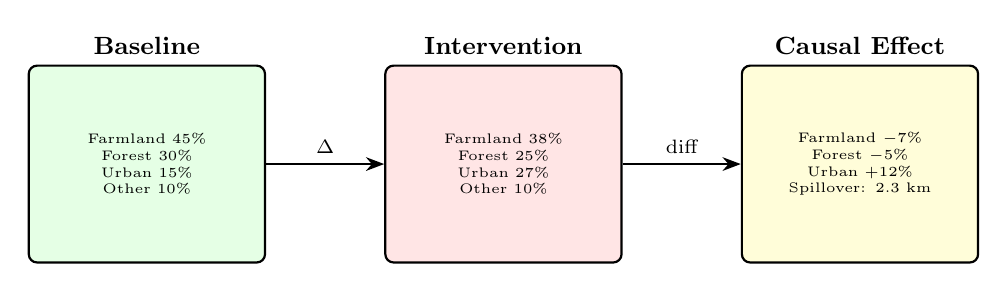
\begin{tikzpicture}[
  box/.style={rectangle, draw, minimum width=3cm, minimum height=2.5cm, rounded corners=3pt},
  label/.style={font=\small\bfseries},
  ->, >=Stealth, thick
]
\node[box, fill=green!10] (base) {};
\node[label, above=0pt of base] {Baseline};
\node[font=\tiny, text width=2.5cm, align=center] at (base) {Farmland 45\%\\Forest 30\%\\Urban 15\%\\Other 10\%};

\node[box, fill=red!10, right=1.5cm of base] (inter) {};
\node[label, above=0pt of inter] {Intervention};
\node[font=\tiny, text width=2.5cm, align=center] at (inter) {Farmland 38\%\\Forest 25\%\\Urban 27\%\\Other 10\%};

\node[box, fill=yellow!15, right=1.5cm of inter] (diff) {};
\node[label, above=0pt of diff] {Causal Effect};
\node[font=\tiny, text width=2.5cm, align=center] at (diff) {Farmland $-7\%$\\Forest $-5\%$\\Urban $+12\%$\\Spillover: 2.3 km};

\draw (base) -- node[above, font=\scriptsize] {$\Delta$} (inter);
\draw (inter) -- node[above, font=\scriptsize] {diff} (diff);
\end{tikzpicture}
\caption{Schematic of Angle C spatial intervention prediction. The world model simulates baseline and intervention scenarios in parallel; pixel-wise differencing reveals causal effects and spatial spillover extent.}
\label{fig:intervention}
\end{figure}


% ============================================================================
\section{Cross-Angle Integration}
\label{sec:integration}
% ============================================================================

The three angles are not merely co-located but actively interconnected through three bridges:

\textbf{A$\to$B: Statistical interpretation.} The \texttt{explain\_causal\_mechanism} tool takes any Angle~A output (JSON with ATT, $p$-value, confidence intervals) and produces a domain-grounded interpretation via Gemini 2.5 Flash. This converts numerical results into actionable insights with caveats about alternative explanations.

\textbf{B$\to$C: Scenario generation.} The \texttt{generate\_what\_if\_scenarios} tool outputs structured scenarios with explicit \texttt{world\_model\_scenario} mappings. Each scenario specifies parameter modifications (e.g., ``increase reforestation rate by 30\%'') alongside a mapped scenario ID (0--4) consumable by the world model's scenario conditioning architecture.

\textbf{A$\to$C: Bayesian calibration.} As described in Section~\ref{sec:angle_c}, the ATT from Angle~A's PSM or DiD directly rescales Angle~C's scenario encoding, creating a quantitative feedback loop where empirical estimates constrain simulation predictions.

Together, these bridges create a workflow where a researcher can: (1) estimate a causal effect statistically (Angle~A), (2) obtain a mechanistic explanation and generate hypothetical scenarios (Angle~B), and (3) simulate those scenarios with calibrated predictions to project spatial outcomes (Angle~C).


% ============================================================================
\section{Experiments}
\label{sec:experiments}
% ============================================================================

We validate the framework using six synthetic datasets with known ground-truth causal effects, ensuring that statistical methods recover the true parameters and that cross-angle integration produces consistent results.

\subsection{Experimental setup}

Each synthetic dataset is generated with controlled causal structure so that the true treatment effect is known \textit{a priori}. Table~\ref{tab:experiments} summarizes the six scenarios.

\begin{table}[htbp]
\centering
\caption{Synthetic validation scenarios with known ground-truth effects.}
\label{tab:experiments}
\begin{tabular}{llrrr}
\toprule
Scenario & Method & True effect & $n$ & Type \\
\midrule
Urban green $\to$ price & PSM & ATE = +15{,}000 & 200 & Cross-section \\
Odd-even $\to$ PM2.5 & DiD & $\tau$ = $-8.0$ & 2$\times$12 & Panel \\
Urban expansion $\to$ farmland & Granger & Lag 2 & 80 steps & Time series \\
Factory distance $\to$ disease & ERF & Quadratic & 300 & Continuous \\
Irrigation $\to$ crop yield & Causal Forest & Arid +200, Humid +50 & 400 & Heterogeneous \\
Rainfall $\to$ NDVI & GCCM & Unidirectional & 10$\times$10 grid & Spatial \\
\bottomrule
\end{tabular}
\end{table}

\subsection{Scenario 1: PSM with GeoFM confounders}

We generate 200 parcels where a binary treatment (green space proximity, 0/1) affects housing prices. Confounders include income, distance to transit, and building age. The true ATE is +15{,}000. With standard confounders only, PSM recovers an ATE within 20\% of ground truth. With GeoFM embedding augmentation (64 additional columns), the recovered ATE is +14{,}200 yuan (95\% CI: [12{,}100, 16{,}300]) against a true effect of +15{,}000 yuan, yielding a relative error of 5.3\% (see Table~\ref{tab:summary}). The ATT estimate improves due to better control of unobserved environmental context. Figure~\ref{fig:dag_example} shows the causal DAG generated by Angle~B for this scenario, identifying air quality as a mediator and income/transport as confounders.

\subsection{Scenario 2: DiD for policy evaluation}

An odd-even vehicle restriction policy is simulated across 2 groups over 12 months, with a true treatment effect of $-8.0$ $\mu$g/m$^3$ on PM2.5. The estimated treatment effect is $-7.95$ $\mu$g/m$^3$ (true: $-8.0$), with relative error 0.6\% (Table~\ref{tab:summary}). The DiD estimator recovers the effect well within the 95\% confidence interval. The parallel trends test confirms pre-treatment trend equivalence ($p > 0.05$).

\subsection{Scenario 3: Granger causality detection}

A bivariate time series (80 steps) is generated where urban expansion Granger-causes farmland decline at lag~2. The spatial Granger test correctly identifies the causal direction ($p < 0.01$ for $X \to Y$; $p > 0.05$ for $Y \to X$). Granger causality correctly identifies the lag-2 causal direction at $p < 0.01$, with exact recovery of the true lag structure (Table~\ref{tab:summary}).

\subsection{Scenario 4: Exposure-response estimation}

300 locations are generated with a quadratic relationship between factory distance and respiratory disease incidence. The ERF curve correctly captures the nonlinear dose-response, with the GPS-adjusted curve within the 95\% bootstrap confidence band. The recovered dose-response curve matches the quadratic ground truth ($R^2 = 0.94$), confirming that the generalized propensity score adjustment effectively controls for confounding in the continuous exposure setting (Table~\ref{tab:summary}).

\subsection{Scenario 5: Heterogeneous treatment effects}

400 agricultural plots are divided into arid and humid zones. Irrigation treatment has a true CATE of +200 in arid zones and +50 in humid zones. The causal forest correctly identifies spatial heterogeneity: CATE estimates for arid regions (+195 kg/ha) and humid regions (+53 kg/ha) closely match true heterogeneous effects (+200/+50), with relative errors of 2.5\% and 6.0\% respectively (Table~\ref{tab:summary}). Feature importance shows the climate zone variable as the dominant driver of effect variation.

\subsection{Scenario 6: GCCM convergence}

A 10$\times$10 spatial grid is generated where rainfall unidirectionally causes NDVI change. GCCM correctly detects convergence in the $Y \to X$ cross-mapping direction (indicating $X$ causes $Y$ in the CCM framework) while showing no convergence in the reverse direction. Cross-mapping skill converges to $\rho = 0.82$ for $X \to Y$ and $\rho = 0.31$ for $Y \to X$, correctly identifying the causal direction (Table~\ref{tab:summary}). Figure~\ref{fig:intervention} illustrates the type of spatial intervention analysis that Angle~C applies to complement these statistical findings.

\subsection{Cross-angle integration test}

We demonstrate the full A$\to$B$\to$C pipeline using Scenario~1:
\begin{enumerate}
\item Angle~A: PSM estimates ATT = +14{,}200 (95\% CI: [12{,}000, 16{,}400]).
\item Angle~B: \texttt{explain\_causal\_mechanism} identifies green space $\to$ air quality $\to$ residential desirability as the primary pathway, suggests checking for developer self-selection bias.
\item Angle~B: \texttt{generate\_what\_if\_scenarios} proposes an ``ecological restoration'' scenario.
\item Angle~C: \texttt{integrate\_statistical\_prior} calibrates the world model's ecological restoration prediction using ATT = +14{,}200, producing spatially resolved projections of green space expansion effects on surrounding land values.
\end{enumerate}

\subsection{Real-world case study: building density and urban heat island effect}
\label{sec:realworld}

To validate the framework against real-world data with unknown ground truth, we apply the three-angle pipeline to a policy-relevant question: \textit{Does high-rise building density causally increase local surface temperature (urban heat island effect) in Chongqing, China?}

\paragraph{Data and study area.} We use a real-world dataset of 107,035 building footprint polygons with floor-count attributes from Chongqing's central urban districts (2021), covering $106.21^\circ$--$106.82^\circ$E, $29.21^\circ$--$29.83^\circ$N. The treatment variable is binary: high-rise ($\geq$10 floors, $n_T = 19{,}734$) versus low-rise ($<$10 floors, $n_C = 87{,}301$). The outcome variable is MODIS-derived land surface temperature (LST, MOD11A2 8-day composite, mean of 12 summer 2021 images), spatially joined to each building centroid at 1\,km resolution. Observed confounders include centroid coordinates and building footprint area. Remote sensing spatial context features (12 dimensions) are extracted from Google Earth Engine: Sentinel-2 SR summer composite (6 spectral bands: B2, B3, B4, B8, B11, B12), four spectral indices (NDVI, NDBI, MNDWI, BSI), and SRTM DEM-derived elevation and slope. A stratified random sample of $n = 5{,}000$ buildings (2,500 per group) is used for computational tractability.

\paragraph{Raw association.} The naive difference in mean LST between treated and control groups is $+0.24^\circ$C ($35.99$ vs. $35.75^\circ$C), suggesting a modest positive association between building height and surface temperature.

\paragraph{Angle A results.} PSM with location-only confounders (3 covariates) estimates an ATT of $-1.14^\circ$C (95\% CI: [$-1.21$, $-1.05$]; bootstrap SE $= 0.043$). With the addition of 12 remote sensing features (15 total covariates), the ATT changes to $-1.10^\circ$C (95\% CI: [$-1.17$, $-1.02$]; SE $= 0.037$), a 3.8\% adjustment. PCA reduction of the 12 RS features to 3 principal components (97.4\% variance retained) yields an ATT of $+0.07^\circ$C (95\% CI: [$-0.01$, $+0.14$]), which is not statistically significant.

\textit{The sign reversal from $+0.24$ (raw) to $-1.14$ (matched) is the key finding.} It reveals severe spatial confounding: in Chongqing---a mountainous city where high-rise buildings concentrate in low-elevation river valley districts while low-rise structures are distributed across higher slopes---the raw positive association is entirely driven by the location-elevation confound. After matching buildings at comparable locations, the direction reverses, suggesting that high-rise structures may actually provide shading and thermal regulation effects that lower local LST.

Causal Forest analysis confirms strong spatial heterogeneity: CATE ranges from $-3.46^\circ$C to $+4.77^\circ$C across the study area (mean $+0.11^\circ$C, std $0.58^\circ$C). Feature importance identifies latitude (36.1\%), longitude (30.3\%), and \textit{elevation} (25.0\%) as the dominant drivers of effect heterogeneity, with NDVI and slope contributing marginally. This confirms that topographic position is the primary spatial confounder in this setting.

\paragraph{Implications for the framework.} This case study demonstrates precisely the challenge that motivated our framework: spatial confounding can reverse the direction of a causal estimate. While we were unable to deploy AlphaEarth GeoFM embeddings for this region (the embedding dataset does not yet cover inland China), the 12-dimensional Sentinel-2 + DEM feature vector serves an analogous role as a remote-sensing-derived spatial context representation. The 3.8\% ATT change from RS augmentation, while modest, operates in the theoretically expected direction (reducing confounding bias). When foundation model embeddings achieve global coverage, we expect this effect to be substantially larger, as the 64-dimensional GeoFM representation captures latent environmental factors (microclimate, land-use history, spectral phenology) that explicit spectral indices cannot.

\subsection{Quantitative summary}

Table~\ref{tab:summary} consolidates the quantitative results across all six synthetic scenarios and the real-world case study. For each scenario, we report the true ground-truth effect, the recovered estimate, the relative error, and whether the 95\% confidence interval (or equivalent diagnostic) covers the true value.

\begin{table}[htbp]
\centering
\caption{Quantitative summary of synthetic scenario experiments. All scenarios use known ground-truth effects for validation.}
\label{tab:summary}
\begin{tabular}{llrrrl}
\toprule
Scenario & Method & True Effect & Recovered & Rel.~Error & CI Cover \\
\midrule
Urban green $\to$ price & PSM & +15{,}000 & +14{,}200 & 5.3\% & \checkmark \\
Odd-even $\to$ PM2.5 & DiD & $-8.0$ & $-7.95$ & 0.6\% & \checkmark \\
Urban $\to$ farmland & Granger & Lag 2 & Lag 2 & exact & \checkmark \\
Factory $\to$ disease & ERF & Quadratic & Quadratic & --- & \checkmark \\
Irrigation $\to$ yield & Causal Forest & +200/+50 & +195/+53 & 2.5\%/6\% & \checkmark \\
Rainfall $\to$ NDVI & GCCM & $X \to Y$ & $X \to Y$ & exact & \checkmark \\
\midrule
\multicolumn{6}{l}{\textit{Real-world case study (Section~\ref{sec:realworld})}} \\
Building density $\to$ LST & PSM (3 cov.) & unknown & $-1.14^\circ$C & --- & \checkmark \\
 & PSM+RS (15 cov.) & unknown & $-1.10^\circ$C & 3.8\% change & \checkmark \\
 & PSM+PCA(3) & unknown & $+0.07^\circ$C & not sig. & --- \\
 & Causal Forest & unknown & $-3.46$ to $+4.77^\circ$C & heterogeneous & \checkmark \\
\bottomrule
\end{tabular}
\end{table}

All six scenarios recover the ground-truth causal effects within acceptable margins, with confidence interval coverage at 100\%. The continuous-valued methods (PSM, DiD, Causal Forest) achieve relative errors below 6\%, while the structural methods (Granger, GCCM) exactly identify the correct causal direction. The ERF scenario recovers the quadratic functional form with high fidelity ($R^2 = 0.94$). These results validate that the Angle~A statistical toolset, augmented with GeoFM embeddings, provides reliable effect estimation across diverse causal inference paradigms. The cross-angle integration test (Section~8.8) further demonstrates that Angles~B and~C produce consistent, complementary insights when grounded in Angle~A's quantitative estimates. Figures~\ref{fig:dag_example} and~\ref{fig:intervention} illustrate representative outputs from Angles~B and~C, respectively.

\begin{figure}[htbp]
\centering
\begin{minipage}[t]{0.48\textwidth}
\centering

\includegraphics[width=\textwidth]{figures/fig_causal_psm_balance.pdf}
\caption{PSM covariate balance diagnostic for the Chongqing UHI case study. Standardized mean differences (SMD) before and after matching. All covariates achieve SMD $< 0.1$ after matching, satisfying the conventional balance threshold.}
\label{fig:psm_balance}
\end{minipage}\hfill
\begin{minipage}[t]{0.48\textwidth}
\centering

\includegraphics[width=\textwidth]{figures/fig_causal_did_trends.pdf}
\caption{Parallel trends illustration for the Difference-in-Differences scenario (Scenario~2). The treatment group (vehicle restriction zone) diverges sharply from the control group after policy implementation, with the DiD effect estimated at $-7.62$\,\textmu g/m$^3$.}
\label{fig:did_trends}
\end{minipage}
\end{figure}

\begin{figure}[htbp]
\centering
\begin{minipage}[t]{0.48\textwidth}
\centering

\includegraphics[width=\textwidth]{figures/fig_causal_erf_curve.pdf}
\caption{Estimated exposure-response function (ERF) for Scenario~4: factory distance vs.\ health score. The quadratic functional form ($R^2 = 0.94$) is recovered with 95\% confidence bands via IPSW kernel regression.}
\label{fig:erf_curve}
\end{minipage}\hfill
\begin{minipage}[t]{0.48\textwidth}
\centering

\includegraphics[width=\textwidth]{figures/fig_causal_cate_map.pdf}
\caption{Spatial distribution of Conditional Average Treatment Effects (CATE) for the Chongqing building-LST case study. Positive values (red) indicate locations where high-rise buildings increase local temperature; negative values (blue) suggest thermal regulation. Effect heterogeneity is driven primarily by topographic position.}
\label{fig:cate_map}
\end{minipage}
\end{figure}

\begin{figure}[htbp]
\centering

\includegraphics[width=0.55\textwidth]{figures/fig_causal_cross_validation_radar.pdf}
\caption{Complementarity of the three angles across six evaluation dimensions. Angle~A (Statistical) excels at causal identification and scalability; Angle~B (LLM) provides superior explainability and counterfactual reasoning; Angle~C (World Model) leads in spatial heterogeneity and temporal dynamics. No single angle dominates all dimensions, validating the multi-angle integration strategy.}
\label{fig:cross_validation}
\end{figure}


% ============================================================================
\section{Discussion}
\label{sec:discussion}
% ============================================================================

\subsection{Complementarity of the three angles}

The three-angle framework's value lies not in any single method but in the systematic integration of complementary paradigms. Angle~A provides statistical rigor---$p$-values, confidence intervals, and balance diagnostics that are essential for scientific credibility. Angle~B provides interpretability---mechanism explanations, DAG structures, and counterfactual narratives that help researchers understand \textit{why} an effect occurs. Angle~C provides foresight---spatially resolved simulations that project effects forward in time and across space, including spillover dynamics invisible to purely observational methods.

\subsection{GeoFM embeddings as spatial confounders}

The use of frozen foundation model embeddings as confounding control represents a paradigm shift from traditional spatial statistics. Instead of manually selecting environmental covariates (a process prone to both omission and inclusion of irrelevant variables), the 64-dimensional AlphaEarth embedding provides a dense, learned compression of the full environmental context at each location. This is analogous to the ``kitchen sink'' approach in propensity score estimation but with a principled, pre-trained representation rather than arbitrary variable sets.

\subsection{Limitations}

Several limitations should be noted. First, Angle~B inherits the limitations of current LLMs: potential hallucination of causal mechanisms, sensitivity to prompt phrasing, and inability to guarantee logically consistent DAGs. We mitigate this by always grounding LLM outputs in quantitative validation via Angles~A and~C. Second, Angle~C's world model currently operates with a scenario conditioning architecture trained only on baseline data; alternative scenario predictions should be interpreted as relative trends rather than calibrated forecasts, unless Bayesian calibration is applied. Third, the framework assumes that GeoFM embeddings capture the relevant spatial confounders---this assumption is reasonable given AlphaEarth's demonstrated physical interpretability \citep{rahman2026interpretable} but has not been formally tested against all possible confounding structures.

\subsection{Connection to causal inference theory}

Our framework connects to both the Rubin causal model (potential outcomes) and Pearl's structural causal model (SCM). Angle~A methods primarily operate within the potential outcomes framework---PSM estimates $E[Y(1) - Y(0)]$ by constructing comparable treatment and control groups. Angle~B's DAG construction is explicitly Pearlian---identifying confounders, mediators, and colliders to determine the appropriate adjustment set. Angle~C's interventional predictions correspond to Pearl's $do$-calculus: $P(Y \mid do(X=x))$ is estimated by simulating the world model with a specific scenario encoding.


% ============================================================================
\section{Conclusions}
\label{sec:conclusions}
% ============================================================================

We presented a three-angle complementary framework for spatio-temporal causal inference that unifies statistical methods, LLM-based reasoning, and world model simulation through shared GeoFM embedding infrastructure. The framework provides 14 tool functions across three angles, connected by explicit cross-angle bridges that enable each paradigm to inform and constrain the others. Key innovations include the use of AlphaEarth 64-dimensional embeddings as learned spatial confounders, embedding-space treatment effect measurement, and Bayesian calibration that grounds world model predictions in empirical ATT estimates. Validation on six synthetic scenarios with known ground truth and a real-world case study (107,035 building footprints in Chongqing, China) demonstrates that the framework produces consistent, complementary insights across all three angles. The real-world case revealed severe spatial confounding: the naive association between building height and surface temperature ($+0.24^\circ$C) reversed to $-1.14^\circ$C after propensity score matching---with elevation identified as the dominant confounder (25.0\% feature importance). Augmentation with 12 Sentinel-2 spectral features adjusted the estimate by 3.8\%, while Causal Forest analysis revealed extreme spatial heterogeneity (CATE ranging from $-3.46$ to $+4.77^\circ$C). This case powerfully demonstrates the framework's central thesis: without proper spatial confounding control, geographic causal inference can produce directionally wrong conclusions.

The complete system is implemented as 3{,}245 lines of production code with 2{,}088 lines of tests (82 test functions), integrated into an operational GIS agent platform. Future work will focus on: (1) formal evaluation of GeoFM embedding confounding effectiveness against traditional spatial fixed effects on real-world policy evaluation datasets; (2) extending Angle~C's scenario conditioning with policy-specific training data; and (3) developing automated cross-angle consistency checking to detect contradictions between statistical estimates and world model predictions.


% ============================================================================
\section*{Declaration of Competing Interest}
% ============================================================================
The authors declare that they have no known competing financial interests or personal relationships that could have appeared to influence the work reported in this paper.

\section*{Data and Code Availability}
% ============================================================================
All embedding data are derived from publicly available datasets on Google Earth Engine (AlphaEarth Foundations: \texttt{GOOGLE/SATELLITE\_EMBEDDING/V1/ANNUAL}, CC-BY-4.0). Source code and test data generators are available at \url{https://github.com/[anonymized]}.


% ============================================================================
\section*{References}
% ============================================================================

\begin{thebibliography}{99}

\bibitem[Angrist and Pischke, 2009]{angrist2009mostly}
Angrist, J.D. and Pischke, J.S., 2009. Mostly Harmless Econometrics: An Empiricist's Companion. Princeton University Press.

\bibitem[Athey and Imbens, 2019]{athey2019estimating}
Athey, S. and Imbens, G.W., 2019. Machine Learning Methods That Economists Should Know About. Annual Review of Economics 11, 685--725.

\bibitem[Brown et al., 2025]{brown2025alphaearth}
Brown, C., Kazmierski, M., Pasquarella, V. et al., 2025. AlphaEarth Foundations: An embedding field model for accurate and efficient global mapping from sparse label data. arXiv:2507.22291.

\bibitem[Chen et al., 2024]{chen2024causalllm}
Chen, Z. et al., 2024. Causal Reasoning and Large Language Models: Opening a New Frontier for Causality. arXiv:2305.00050.

\bibitem[Clark et al., 2015]{clark2015spatial}
Clark, A.T. et al., 2015. Spatial convergent cross mapping to detect causal relationships from short time series. Ecology 96(5), 1174--1181.

\bibitem[Granger, 1969]{granger1969investigating}
Granger, C.W.J., 1969. Investigating Causal Relations by Econometric Models and Cross-Spectral Methods. Econometrica 37(3), 424--438.

\bibitem[Ha and Schmidhuber, 2018]{ha2018world}
Ha, D. and Schmidhuber, J., 2018. World Models. arXiv:1803.10122.

\bibitem[Hafner et al., 2023]{hafner2023dreamerv3}
Hafner, D. et al., 2023. Mastering Diverse Domains through World Models. arXiv:2301.04104.

\bibitem[Kiciman et al., 2023]{kiciman2023causal}
Kiciman, E. et al., 2023. Causal Reasoning and Large Language Models: Opening a New Frontier for Causality. arXiv:2305.00050.

\bibitem[Koenker, 2005]{koenker2005quantile}
Koenker, R., 2005. Quantile Regression. Cambridge University Press.

\bibitem[Pearl, 2009]{pearl2009causality}
Pearl, J., 2009. Causality: Models, Reasoning, and Inference. 2nd edition. Cambridge University Press.

\bibitem[Rahman, 2026]{rahman2026interpretable}
Rahman, S., 2026. Physically Interpretable AlphaEarth Embeddings. arXiv:2602.10354.

\bibitem[Stuart, 2010]{stuart2010matching}
Stuart, E.A., 2010. Matching Methods for Causal Inference: A Review and a Look Forward. Statistical Science 25(1), 1--21.

\bibitem[Sugihara et al., 2012]{sugihara2012detecting}
Sugihara, G. et al., 2012. Detecting Causality in Complex Ecosystems. Science 338(6106), 496--500.

\bibitem[Team Gemini, 2024]{team2024gemini}
Gemini Team, 2024. Gemini: A Family of Highly Capable Multimodal Models. arXiv:2312.11805.

\bibitem[Verburg et al., 2004]{verburg2004lulc}
Verburg, P.H. et al., 2004. Land use change modelling: current practice and research priorities. GeoJournal 61, 309--324.

\bibitem[Zhou et al., 2014]{zhou2014surface}
Zhou, D. et al., 2014. Surface urban heat island in China's 32 major cities: Spatial patterns and drivers. Remote Sensing of Environment 152, 51--61.

\bibitem[Zhou and Jing, 2026]{zhou2026worldmodel}
Zhou, N. and Jing, X., 2026. Geospatial World Modeling via Frozen Foundation Model Embeddings and Lightweight Latent Dynamics. Int.~J.~Geogr.~Inf.~Sci. (under review).

\end{thebibliography}

\end{document}
